% Radioactivity

\documentclass[11pt]{article}

\usepackage[a4paper, margin=1in]{geometry}

\usepackage{amsmath}

\usepackage{amssymb}

\usepackage[german]{babel}

\usepackage[autostyle=true]{csquotes}

\usepackage{libertine}

\usepackage[libertine]{newtxmath}

\usepackage{tikz}

\usepackage{gensymb}

\usepackage{fancyhdr}

\usepackage{amsfonts}

\usepackage{pgfplots}

\pgfplotsset{compat=1.10}

\usepackage{multicol}

\usepackage{caption}

\usepackage{floatrow}

\everymath{\displaystyle}

% Header / footer settings

\pagestyle{fancy}
\fancyhf{}
\renewcommand{\headrulewidth}{0.2mm}
\fancyhead[C]{Funktionen}
\renewcommand{\footrulewidth}{0.2mm}
\fancyfoot[L]{Peter Goldsborough}
\fancyfoot[C]{\thepage}
\fancyfoot[R]{\today}

\fancypagestyle{plain}{%
	\fancyhf{}
	\renewcommand{\headrulewidth}{0mm}%
	\renewcommand{\footrulewidth}{0.2mm}%
	\fancyfoot[L]{Peter Goldsborough}
	\fancyfoot[C]{\thepage}
	\fancyfoot[R]{\today}
}


\setlength{\headheight}{15pt}

\setlength{\parindent}{0pt}

\addtolength{\parskip}{\baselineskip}


\newcommand{\overbar}[1]{\mkern 1.5mu\overline{\mkern-1.5mu#1\mkern-1.5mu}\mkern 1.5mu}

\newcommand{\heading}[1]{\begin{center}\Huge \textbf{#1}\end{center}\par}

\newcommand{\sub}[1]{\vspace{\parskip}{\LARGE\textbf{#1}}}

\newcommand{\subsub}[1]{{\Large \textbf{#1}}}

\newcommand{\subsubsub}[1]{\textbf{#1}}

\newcommand{\colvec}[1]{\begin{pmatrix}#1\end{pmatrix}}

\newcommand{\extrapar}{\par\vspace{\baselineskip}}

\newcommand{\zitat}[1]{\foreignquote{german}{#1}}

\newcommand{\bolditem}[1]{\item \textbf{#1}}

\newcommand{\titleitem}[1]{\bolditem{#1}\par}

\newcommand{\defas}{ \dots \,\,}

\begin{document}

\title{\Huge Radioactivity}

\author {
Peter Goldsborough\\
8A
}

\date{\today}

\maketitle

\chapter*{Properties of Alpha, Beta and Gamma Radiation}

\section*{Ionization}

First, it should be discussed what ionizing radiation and ionization is in general. Ioniziation is the process in which an electron of an atom is given enough energy to break away from the atom, yielding two charged particles (ions): the now positively charged atom and the free electron. This ionzation may be induced either directly, by ions such as $\alpha$ or $\beta$ particles, which interact via electrostatic forces of attraction and repulsion due to their charge, or indirectly through electromagnetic waves such as $\gamma$ radiation, which may transfer enough energy to the electron upon collision for the electron to break free.

\section*{Alpha $\alpha$}

Alpha radiation is a form of particle radiation. occuring when an unstable radioactive nucleus is too heavy. Alpha particles are composed of two neutrons and two protons, whose total mass is 7000 times that of $\beta$ particles. Because of its two protons, it has a charge of $+2$. Moreover, it should be mentioned that alpha particles have exactly the same atomic structure as a Helium atom. Therefore, alpha particles are either denoted by $\alpha^{2+}$ or $He^{2+}$. In air, its speed is one twentieth of the speed of light. Alpha particles are deflected in an electric field because of their charge, which attracts them to the field's negative side. Due to the Lorentz force, they are also deflected in a magnetic field. Moreover, alpha particles cause ionization because of their charge. Alpha radiation generally does not penetrate the skin, however, it can penetrate thin tissue such as open wounds or eyes. The biggest risk stems from internal damage, by ingesting alpha particles, which can cause cancer. In general, alpha particles have a low penetration depth, so it can be even stopped by air.

\pagebreak

\section*{Gamma $\gamma$}

Gamma radiation is a form of electromagnetic wave radiation. $\gamma$-rays have very high energy --- in the region of keV or MeV --- and frequency --- about $10^{20} Hz$ --- and travel at the speed of light, as it is an electromagnetic wave. It follows alpha or beta decay, often because said decay caused a change in element. More specifically, $\gamma$ radiation occurs when the energy of an unstable radioactive nuclide is still too high, so that it must emit its excess energy in form of a gamma ray. Consequently, the atom goes from an unstable, excited state to a state of higher stability and lower energy, caused by the $\gamma$ radiation, which is also a form of quantum jump. As a gamma ray is a wave, it has neither mass nor does it carry any charge. However, it can still cause ionization when it collides with atoms. A $\gamma$-ray is deflected neither in an electric nor in a magnetic field, due to the fact that it carries no charge. Gamma rays travel with high energy, speed and penetration depth. They can only be dampened --- not stopped entirely --- by lead.

\section*{Beta $\beta$}

Beta radiation is also a form of particle radiation. There are in fact two forms of beta radiation, $\beta^-$ and $\beta^+$.

 Beta minus ($\beta^-$) particles are identical to electrons and carry a charge of $-1$, however, they originate from inside the nucleus and not from the energy levels outside, as normal electrons do. Beta minus particles are formed when the ratio of neutrons to protons in an atom is too high, causing a neutron to transform into an electron $e^-$, a proton $p^+$ and an electron anti-neutrino $\bar{\nu_{e}}$. The electron is then emitted as the $\beta^-$ particle, while the proton is kept. Thus, the neutron count is reduced by one and the proton count increased by one.

The second variant of beta decay is called $\beta^+$ or \emph{positron} emission ($e^+$). It occurs for the opposite reason of $\beta^-$ decay, namely to reduce the proton count and increase the neutron count by one. In this case, a proton $p^+$ transforms into a neutron $n$, a positron --- denoted by $e^+$ or $\beta^+$ --- and an electron neutrino $\nu_{e}$. Because the proton count decreases, the atomic number of the element decreases while the mass number stays the same.

Because the number of neutrons determines the element of an atom, beta radiation can change an atom to another element. This is called $\beta$-decay. Because a beta particle is charged either way ($\beta^-$ and $\beta^+$), it is deflected in an electric field (attracted by the side of the opposite charge) and also in a magnetic field. Beta particles cause ionization upon colliding with other atoms. Beta particles move at about half the speed of light. Beta particles travel faster and longer than $\alpha$-particles and have a higher penetration depth. They can penetrate the skin, but can be stopped by an aluminium plate.

\chapter*{Detecting Radioactivity}

Geiger-Muller tubes work by directing particle ($\alpha$ and $\beta$) or electromagnetic wave ($\gamma$) radiation through a mica-window (very thin, to let through $\alpha$ particles) into a tube filled with Argon or any other unreactive noble gas. The radioactive particles collide with Argon atoms, which are ionized and eject electrons as a consequence. An avalanche effect causes ionization of the gas when ejected electrons collide with other atoms, ionizing more and more atoms. An electric field with opposite charges is formed --- turning the gas into plasma. This is the ``ionizing effect''. The case of the tube is charged negatively and an anode is placed inside the tube. When no radiation ionizes the gas, no current flows between the case and the anode. However, when the gas is ionized, it can conduct the current from the case to the anode. The voltage produced is measured by the G-M Counter and is converted into a value and as well as acoustic signal. Figure \ref{fig:gm} displays a G-M Counter apparatus.

\begin{figure}[b!]
  \vspace{\baselineskip}
  \centering
  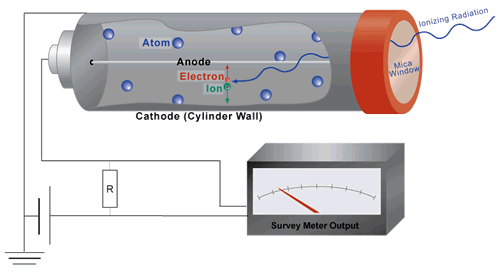
\includegraphics[scale=0.8]{img/gm}
  \caption{A Geiger-Muller Counter}
  \label{fig:gm}
\end{figure}

The \emph{activity} of radioactive nuclei is measured in Becquerel [Bq], where one Bq is equivalent to the decay of one nucleus per second.

\pagebreak

\chapter*{Radioactive Decay}

Radioactive decay is the process by which an unstable radioactive nuclide undergoes either $\alpha, \beta$ or $\gamma$ decay to transform or \emph{decay} into a different isotope of the same element, or to a different element entirely. Radioactive decay always occurs inside of an atom's nucleus and never in any of its surrounding energy levels. Moreover, the decay of a radionuclide is a completely random event and can be influenced neither by physical nor by chemical processes. Lastly, it should be noted that the decay of an unstable radioactive nuclide to a stable atom causes its potential energy to decrease, as it is less likely that an atom that has already undergone decay will do so again.

Generally, only nuclei which can reach a lower energy state by sending out radiation are radioactive.

\section*{Half-life}

The half-life of a radioactive particle sample is the time after which half the nuclei of the sample will have undergone radioactive decay.

Figure \ref{fig:decay} shows the decay curve for 1 million Carbon-14 nuclei, which have a half-life of 5700 years, for the first 28 500 years.

\begin{figure}[h!]
\centering
  \begin{tikzpicture}
    \begin{axis}
    [
      xlabel = $t$,
      ylabel = $N(t)$,
      grid = both,
      samples = 1000,
      domain = 0:32000,
      axis lines = middle,
      scaled y ticks = false,
      scaled x ticks = false,
      y tick label style={/pgf/number format/fixed},
      x tick label style={/pgf/number format/fixed},
      xtick = {0, 5700, 11400, 17100, 22800, 28500}
    ]

      \addplot [mark=*, black]
      coordinates 
      {
        (0, 1000000)
        (5700, 500000)
        (11400, 250000)
        (17100, 125000)
        (22800, 62500)
        (28500, 31250)
      };

    \end{axis}
  \end{tikzpicture}
\caption{The decay curve of Carbon-14, where $t$ is time in years}
\label{fig:decay}
\end{figure}

\pagebreak

\section*{Alpha $\alpha$}

Alpha decay takes place when the nucleus of an atom is too heavy, making it necessary to emit some of its nucleons as an $\alpha^{2+}$ particle, which consists of two protons and two neutrons. Given that the number of neutrons and protons determines the mass and atomic number of an element, it is clear that Alpha decay causes the radioactive nuclide to decay either to a different isotope of the same element, or to a different element entirely.

Equation \ref{eq:alpha1} shows the decay equation for the alpha decay of Radium-226 and Equation \ref{eq:alpha2} that for Radium-222.

\begin{equation}
  \ce{^{226}_{88}Ra} \rightarrow \ce{^{222}_{86}Rn} + \ce{^{4}_{2}\alpha}
  \label{eq:alpha1}
\end{equation}

\begin{equation}
  \ce{^{222}_{86}Ra} \rightarrow \ce{^{218}_{82}Rn} + \ce{^{4}_{2}\alpha}
  \label{eq:alpha2}
\end{equation}

\subsection*{Details}

It should be investigated why Alpha radiation is possible in the first place. Under the laws of classical physics, nucleons (protons and neutrons) are trapped inside the nucleus of an atom and have no means to overcome the strong nuclear force --- the attractive force acting between nucleons and binding them inside the nucleus, overcoming the electrostatic repulsion between protons. However, Quantum Mechanics introduces a set of new paradigms by which to judge phenomena such as alpha radiaton. According to Heisenberg's uncertainty principle of time and energy, it would be possible that for a very short, unobservable period of time, the $\alpha$ particles inside the nucleus could borrow enough energy to overcome the strong nuclear force and radiate out of the nucleus, subsequently releasing the borrowed energy. The source of the borrowed energy is the left-over energy from the mass defect $\Delta m$ of the last decay the nucleus underwent, which was converted into energy according to $E = mc^2$. 

Equation \ref{eq:heisenberg} shows Heisenberg's uncertainty principle of time and energy, where $\Delta E$ is the deviation in observed energy of the particle, $\Delta t$ the deviation in time of the observation and $h$ Planck's constant. 

\begin{equation}
  \Delta E \cdot \Delta t \geq \frac{h}{4\pi}
  \label{eq:heisenberg}
\end{equation}

The basic message of Heisenberg's uncertainty principle and the equation shown above is that to measure the energy of a particle at any given moment precisely, one would need a considerable amount of time to perform that measurement. Therefore, $\Delta E$ would be small, as the measurement would not deviate much from the real value given the large measurement period. However, it would be impossible to say precisely at what instant of time the particle took on that specific energy value, given that the time window was large. Thus $\Delta t$ would also be large, as the measured time deviates from the real time (at which the particle took on that specific energy value) by a considerable amount.

On the other hand, and more important for the topic of alpha radiation and tunneling, if the time interval of the measurement performed is small, the deviation in time $\Delta t$ of any measurement will automatically be smaller, as there is simply less room (i.e. time) for error. However, it will be more difficult to perform an exact measurement if there is less time to do so. Thus, $\Delta E$ is large. 

Given this explanation, it can be said that hypothetically, an alpha particle could borrow energy in a time interval $\Delta t$ so unmeasureably small that the deviation in energy $\Delta t$ could be massive, possibly giving the particle enough energy to overcome the strong nuclear force and ``tunnel'' through the Coulomb Barrier (see below).

\begin{figure}[h!]
  \centering
  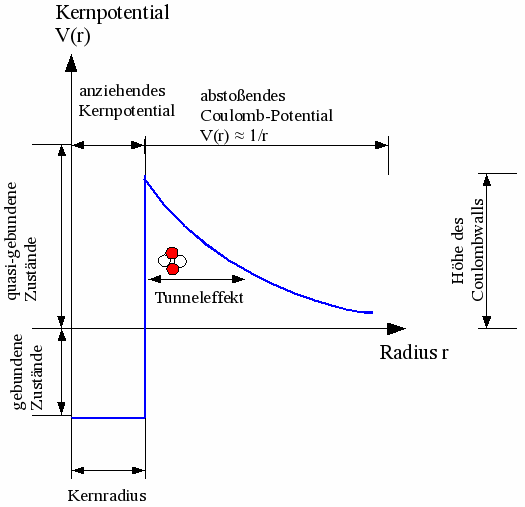
\includegraphics[scale=0.7]{img/coulomb}
  \caption{Representation of the Coulomb Barrier inside of a nucleus}
  \label{fig:coulomb}
\end{figure}

The Coulomb Barrier and the curve shown is the barrier in energy an alpha particle must reach or surpass to radiate out of the nucleus and release itself from the grip of the strong nuclear force, which normally binds the particles together at the core of the atom. 

The energy a particle holds can be seen as its potential energy --- or \emph{nuclear potential}. A higher nuclear potential (= more energy) means a higher probability that the particle will radiate out of the nucleus at any given point in time. Moreover, also the width and height of the Coulomb Barrier determines the nuclear potential, as a particle requires less energy to radiate out if the threshold energy is lower. Therefore, these two factors --- the base energy value held by the nucleons and the dimensions of the Coulomb Barrier --- determine the rate of decay and the half-life of a radionuclide. A lower nuclear potential means less probability for decay and thus a lower half-life. A higher nuclear potential, either due to a higher base energy held by nucleons from converted energy of the last decay's mass defect, or due to a lower Coulomb Barrier to overcome (more nucleons = more nucleons to bind with same amount of energy = weaker overall force acting on each individual nucleon), indicates a higher probability for decay and thus a shorter half-life, as half the nuclei of any given sample decay more quickly. 

\pagebreak

The aforementioned tunneling phenomenon can now be visualized as the event whereby the alpha particle borrows enough energy at an unmeasurable point in time to overcome the Coulomb Barrier even though its nuclear potential does not yet suffice to overcome the barrier without that borrowed energy.

Lastly, the terms ``bound'', ``quasi-bound'' and ``free'' should be examined:

\begin{itemize}
  \item \textbf{bound}: When a particle has no base energy and does not have a positive nuclear potential (below x axis in graph). Is held back by strong nuclear force in all cases.

  \item \textbf{quasi-bound}: When a particle has positive base energy (from converted mass defect energy of last decay), but not enough to overcome the Coulomb Barrier. Were there no strong nuclear force, such a particle would be free.

  \item \textbf{free}: When a particle has enough positive base and borrowed energy to either overcome or tunnel through the Coulomb Barrier and be free and unaffected by the strong nuclear force.
\end{itemize}

\section*{Beta $\beta$}

Beta decay occurs when a radionuclide's neutron-to-proton ratio is imbalanced. Depending on whether the unstable radioactive nuclide requires more neutrons or more protons to become stable, either a neutron is transformed to a proton, a $\beta^-$ particle and an electron anti-neutrino ($\beta^-$ decay) or, the other way around, a proton is transformed into a neutron, a $\beta^+$ particle, i.e. a \emph{positron}, and an electron neutrino ($\beta^+$ decay). Either way, the ratio and thus the nucleus is stabilized as necessary.

\subsection*{$\beta^-$ Decay}

In a radioactive nucleus undergoing $\beta^-$ decay, a neutron $n$ is transformed into a $\beta^-$ particle, which is simply an electron ($e^-$), a proton $p^+$ as well as an electron anti-neutrino $\bar{\nu_{e}}$. The latter must be present because the mass of the electron and proton released do not equal that of the original neutron, thus the electron anti-neutrino must be responsible for containing the remaining mass in its energy, according to Eintein's mass-energy relationship $E = mc^2$. A general $\beta^-$ decay equation for a free neutron $n$ is therefore: $$n \rightarrow p^+ + \beta^- + \bar{\nu_{e}}$$

Given that for $\beta^-$ decay the neutron count decreases and the proton count increases by one, it can be said that during $\beta^-$ decay, the mass number stays the same, as a neutron is exchanged for a proton, while the atomic / proton number increases by one.

Equation \ref{eq:beta1} shows the decay equation for the $\beta^-$ decay of Polonium-218 and Equation \ref{eq:beta2} for Carbon-14.

\begin{equation}
  \ce{^{218}_{84}Po} \rightarrow \ce{^{218}_{85}As} + \beta^- + \bar{\nu_{e}}
  \label{eq:beta1}
\end{equation}

\begin{equation}
  \ce{^{14}_{6}C} \rightarrow \ce{^{14}_{7}N} + \beta^- + \bar{\nu_{e}}
  \label{eq:beta2}
\end{equation}

\subsection*{$\beta^+$ decay}

Contrary to $\beta^- decay$, beta plus decay does not involve the transformation of a neutron to a proton, but in fact the other way around. Therefore, it can be said that during $\beta^+$ decay, a proton $p^+$ is converted into a neutron $n$, a $\beta^+$ particle, which is equivalent to a positron $e^+$, as well as an electron neutrino $\nu_{e}$, again for reasons of mass and energy conservation laws: $$p^+ = n + \beta^+ + \nu_{e}$$

\subsubsection*{Details}

It should be mentioned that, on the one hand, the $\beta^-$ (= electron $e^-$) and electron anti-neutrino $\bar{nu_{e}}$ particles released during $\beta^-$ decay, and, on the other hand, the $\beta^+$ (= positron $e^+$) and electron neutrino $\nu_{e}$ released during $\beta^+$ decay, are \emph{anti-particles} of each other. This means that if two respective anti-particles collide, they annihilate and are transformed into $\gamma$ rays and thus into energy. This gives insight into why the particles released during $\beta^+$ and $\beta^-$ decay are specifically the ones mentioned above. The reason why is that either form of decay must be fully reversible to be in accordance with the laws of physics. Given an equation for $\beta^-$ decay, it should be considered what happens when the newly created proton $p^+$ undergoes the reverse decay equation which is $\beta^+$ decay: 

\begin{table}[h!]
\centering
  \begin{tabular}{l l l}
    \underline{n} & $\to$ & $p^+ + \bcancel{\beta^-} + \bcancel{\bar{\nu_{e}}}$
    \\
    && $p^+$ $\to  \text{\underline{n}} + \bcancel{\beta^+} + \bcancel{\nu_{e}}$
  \end{tabular}
\end{table}

As can be seen, the particles created during the $\beta^-$ decay in the first line (electron / $\beta^-$ and electron anti-neutrino) cancel out with their anti-particles created from the subsequent $\beta^+$ decay (positron / $\beta^+$ and electron neutrino). The result of the second decay is again a neutron (underlined), thus proving that the two decays are perfect anti-reactions to each other, having neutralized all other particles.

\section*{Gamma $\gamma$}

Gamma decay involves the emission of a $\gamma$ ray from the nucleus of an unstable radioactive atom. Because Gamma decay does not affect the nucleons of the atom and changes neither the neutron nor the proton count, the mass and atomic numbers and thus the element of the atom stay the same during and after $\gamma$ decay. The only change is that the atom goes from a high-energy, excited to a more stable, lower-energy state by emitting the quantum of energy that is a gamma ray. 

Equation \ref{eq:gamma} shows the decay equation for the $\gamma$ decay of Cobalt-99, where $m$ denotes an excited or \emph{metastable} state.

\begin{equation}
  \ce{^{99m}_{43}Tc} \rightarrow \ce{^{99}_{43}Tc} + \gamma
  \label{eq:gamma}
\end{equation}

\pagebreak

\section*{Applications of radioactive isotopes}

\begin{itemize}
  \item Smoke detectors
  \item Medical uses
  \item Irradiation in Pest Control
  \item Archeological dating
  \item Agricultural uses
\end{itemize}

\section*{Nuclear medicine}

A nowadays popular use of radioactivity is nuclear medicine and specifically medical imaging, for which radioactive substances are used as \emph{tracers}.

\subsection*{Tracers}

A tracer is a sample of a radioactive isotope used in medical imaging that is injected into a medical patient to measure his or her metabolic pathways and blood flow. The radioisotope used, often Iodine-131 or Technetium-99, emits $\beta$ or $\gamma$ radiation, as only these two forms of radiation can penetrate tissue, especially $\gamma$ radiation, which has a very high penetration depth without decrease in intensity. In contrast, $\alpha$ radiation can be stopped very easily by tissue or paper and is thus unsuited for detection. Moreover, the radioisotope chosen must have a short half-life (e.g. 8 days for I-131, 6 hours for Tc-99), to minimize the radiation dose and radioactive exposure and thus the harm caused to the medical patient. The radiation produced can be detected by external detection apparati to trace the flow and accumulation points of the radionuclide.

\subsection*{Scintigraphy}

In Scintigraphy, a sample of a radioactive tracer is bound to a certain molecular carrier compound known to bind to the tissue of the body region of interest within the medical patient (e.g. kidney). This tracer is then introduced into the body via a radiopharmaceutical or injected into the blood stream of the patient, so that its flow and accumulation regions may be observed by detecting the radiation produced by the decay of the radioisotopes. The observation data is then converted into a 2D color image of the body (as opposed to PET, where a 3D image is produced).

\subsection*{Positron-Emission-Tomography (PET)}

In Positron-Emission-Tomography (PET), $\beta^+$ or \emph{positron} ($e^+$) emitting radioisotopes such as Carbon-11 or Fluorine-18 are introduced into the body of the medical patient via a radiopharmaceutical or direct injection or inhalation. These radioisotopes are bound to molecular carrier compounds known to be taken up by the tissue of the body organ / tissue of interest, such as glucose molecules for cancerous tissue regions, so that the molecule together with the radionuclide may accumulate in those specific regions. When the unstable radioactive nucleus undergoes $\beta^+$ decay, a proton is converted into a neutron, a $\beta^+$, particle which is equivalent to a positron $e^+$, and an electron neutrino $\nu_{e}$. The $\beta^+$ particle is emitted and soon collides with an electron in its path. Because a $\beta^+$ particle is a positron ($e^+$), which is the anti-particle of an electron ($e^-$), the two (anti-)particles annihilate and transform into two $\gamma$ photons upon collision. The energy of the gamma rays was found to be 511 keV, which can be determined via Einstein's mass-energy-relationship $E=mc^2$. The two $\gamma$ rays produced travel in opposite directions due to momentum conservation laws and exit the body of the patient, as $\gamma$ rays have a high penetration depth and can easily cross the patient's body tissue with little loss in intensity. The patient undergoing PET is lying in a ring of detectors, which detect the two $\gamma$ photons comming out of the patient on the same line in space, at opposite sides of the body. By calculating the intersection points between the many lines from many different $\beta^+$ decays, the computer detecting the radiation can compute regions of high intensity within the body, which it visualizes on a 3D-image.

\end{document}
